\documentclass[border=0.8ex,svgnames,tikz]{standalone}
\usepackage{amsmath,mathtools}
\usepackage{fontspec}
\setmainfont{Source Serif 4}
\setsansfont{Source Sans 3}
\setmonofont{Source Code Pro}
\usepackage{ifthen}
\usetikzlibrary{positioning,chains,shapes.multipart}
\begin{document}
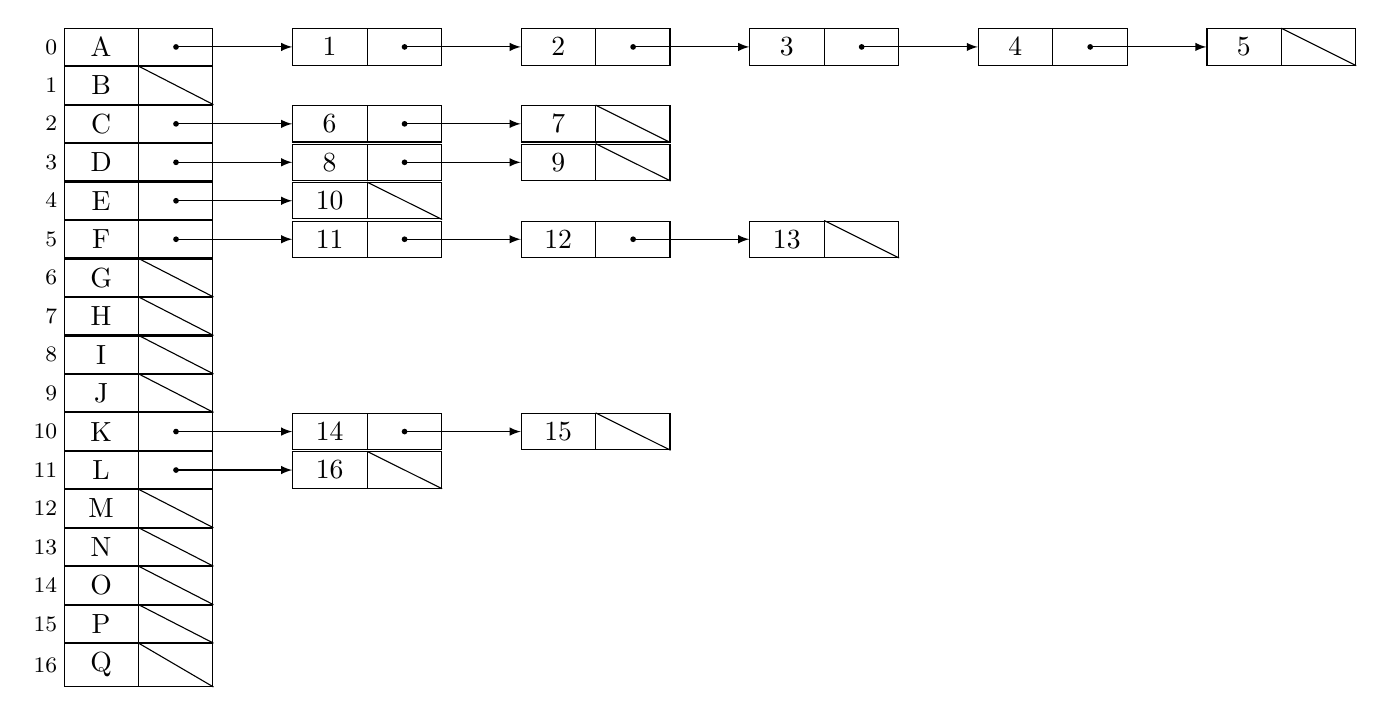
\begin{tikzpicture}
  \begin{scope}[
    every node/.style={
      draw,
      on chain,
      align=center,
      rectangle split,
      rectangle split horizontal,
      rectangle split parts=2,
      rectangle split every empty part={},
    },
    every one node part/.style={text width=2em,text height=1em,text
      depth=0.32em},
    every two node part/.style={text width=2em,text height=1em,text
      depth=0.32em},
    ]
    \begin{scope}[start chain=going below,node distance=0]
      \foreach[count=\i from 0] \val/\haschild in
      {A/1,B/0,C/1,D/1,E/1,F/1,G/0,H/0,I/0,J/0,K/1,L/1,M/0,N/0,O/0,P/0,Q/0}
      {
        \node(node\i){ \nodepart{one}\val \nodepart{two}{} };
        \coordinate(node\i-center) at (node\i.two south|-node\i.two east);
        \ifthenelse{\haschild=1}{
          \path[fill=Black] (node\i-center) circle (0.24ex);
        }{
          \path[draw] (node\i.south east) -- (node\i.north);
        };
        \chainin(node\i);
      }
    \end{scope}
    \begin{scope}[start chain=going right]
      \foreach[evaluate=\xtmp using {int(\x+\n)},remember=\xtmp as \x] \i/\n in
      {0/5,2/2,3/2,4/1,5/3,10/2,11/1}
      {
        \chainin(node\i);
        \pgfmathtruncatemacro{\xbegin}{\x+1};
        \pgfmathtruncatemacro{\xend}{\x+\n};
        \foreach \xval in {\xbegin,...,\xend}{
          \node(node\i\xval){ \nodepart{one}\xval \nodepart{two}{} };
          \ifthenelse{\xval=\xbegin}
          { \path[draw,->,>=latex] (node\i-center) -- (node\i\xval); }
          {}
        }
        \foreach \xval in {\xbegin,...,\xend}{
          \pgfmathtruncatemacro{\xnext}{\xval+1};
          \begin{scope}[node distance=0]
            \coordinate(node\i\xval-center) at (node\i\xval.two
            south|-node\i\xval.two east);
          \end{scope}
          \ifthenelse{\xval=\xend}{
            \path[draw] (node\i\xval.south east) -- (node\i\xval.north);
          }{
            \path[fill=Black] (node\i\xval-center) circle (0.24ex);
            \path[draw,->,>=latex] (node\i\xval-center) -- (node\i\xnext);
          };
        }
      }
    \end{scope}
  \end{scope}
  \begin{scope}[
    every node/.style={
      draw=none,
      align=center,
      font=\footnotesize,
      inner sep=0.5ex,
    },
    node distance=0,
    ]
    \foreach \i in {0,...,16}
    {
      \node[left=of node\i]{\i};
    }
  \end{scope}
\end{tikzpicture}
\end{document}
